Our long-context solution consists of a continual pretraining and a finetuning phase, both are light-weight.
We hold the basic hypothesis that the potential of utilizing information anywhere within the 200K input context is already 
exist in the base model (same as~\citealt{fu2024data}), the continue pretraining phase ``unlocks'' such capability, evidenced by a strong performance on Needle-in-a-Haystack test, then the finetuning phase further adapt the style of response to follow human instruction and preference. 

\textbf{Continue Pretraining}\quad
We continue pretrain the full-attention model using sequence parallelism~\citep{li2021sequence} and distributed attention.
This is to say, we do not use any sparse or linear attention, but use a brute force implementation of the full attention.
We continue pretrain the Yi 6B/ 34B base model on the data mixture of 
(1). original pretraining data, as is introduced in section~\ref{sec:pretrain}; 
(2). length-upsampled long-context data, where the long documents are mostly from books; 
(3). multi-document question-answering synthetic data, where we construct QA pairs where the answer contains a recitation of the related paragraph before the answer. 
Our data approach mostly follows the data engineering practice in~\citet{fu2024data} and~\citet{yu2023paraphrasing}. 
We continue pretrain the model on 5B tokens with 4M batch size, which translate to 100 optimization steps.
Aligning with the concurrent work from~\citet{fu2024data}, we observe that such light-weight continue pretraining is already able to enable a strong performance on Needle-in-a-Haystack test, as we will show in Figure~\ref{fig:needle}. 

\textbf{Supervised Finetuning}\quad
We mix our short-context SFT data with long-context document question-answering data. 
We use model-assisted automated methods (i.e., synthetic data) to construct document QA.
Specifically, we randomly concatenate multiple documents into a sequence, sample one or more paragraphs from the long sequence, and ask a chat model to construct question and answer pairs based on the sampled paragraph.
One important detail is recitation and rephrasing: before giving the answer, we ask the model to recite or paraphrase the original paragraph. 
This data format encourages the model's retrieval behavior and consequently discourages the hallucination behavior: given a question, the model is more likely to use the information within the input to construct the answer, rather than use its internal knowledge, which may be related but inaccurate. 
Our finetuned model is deployed at \url{www.wanzhi01.com}, and we encourage the readers to try it out. 

\begin{figure}
	\begin{center}
		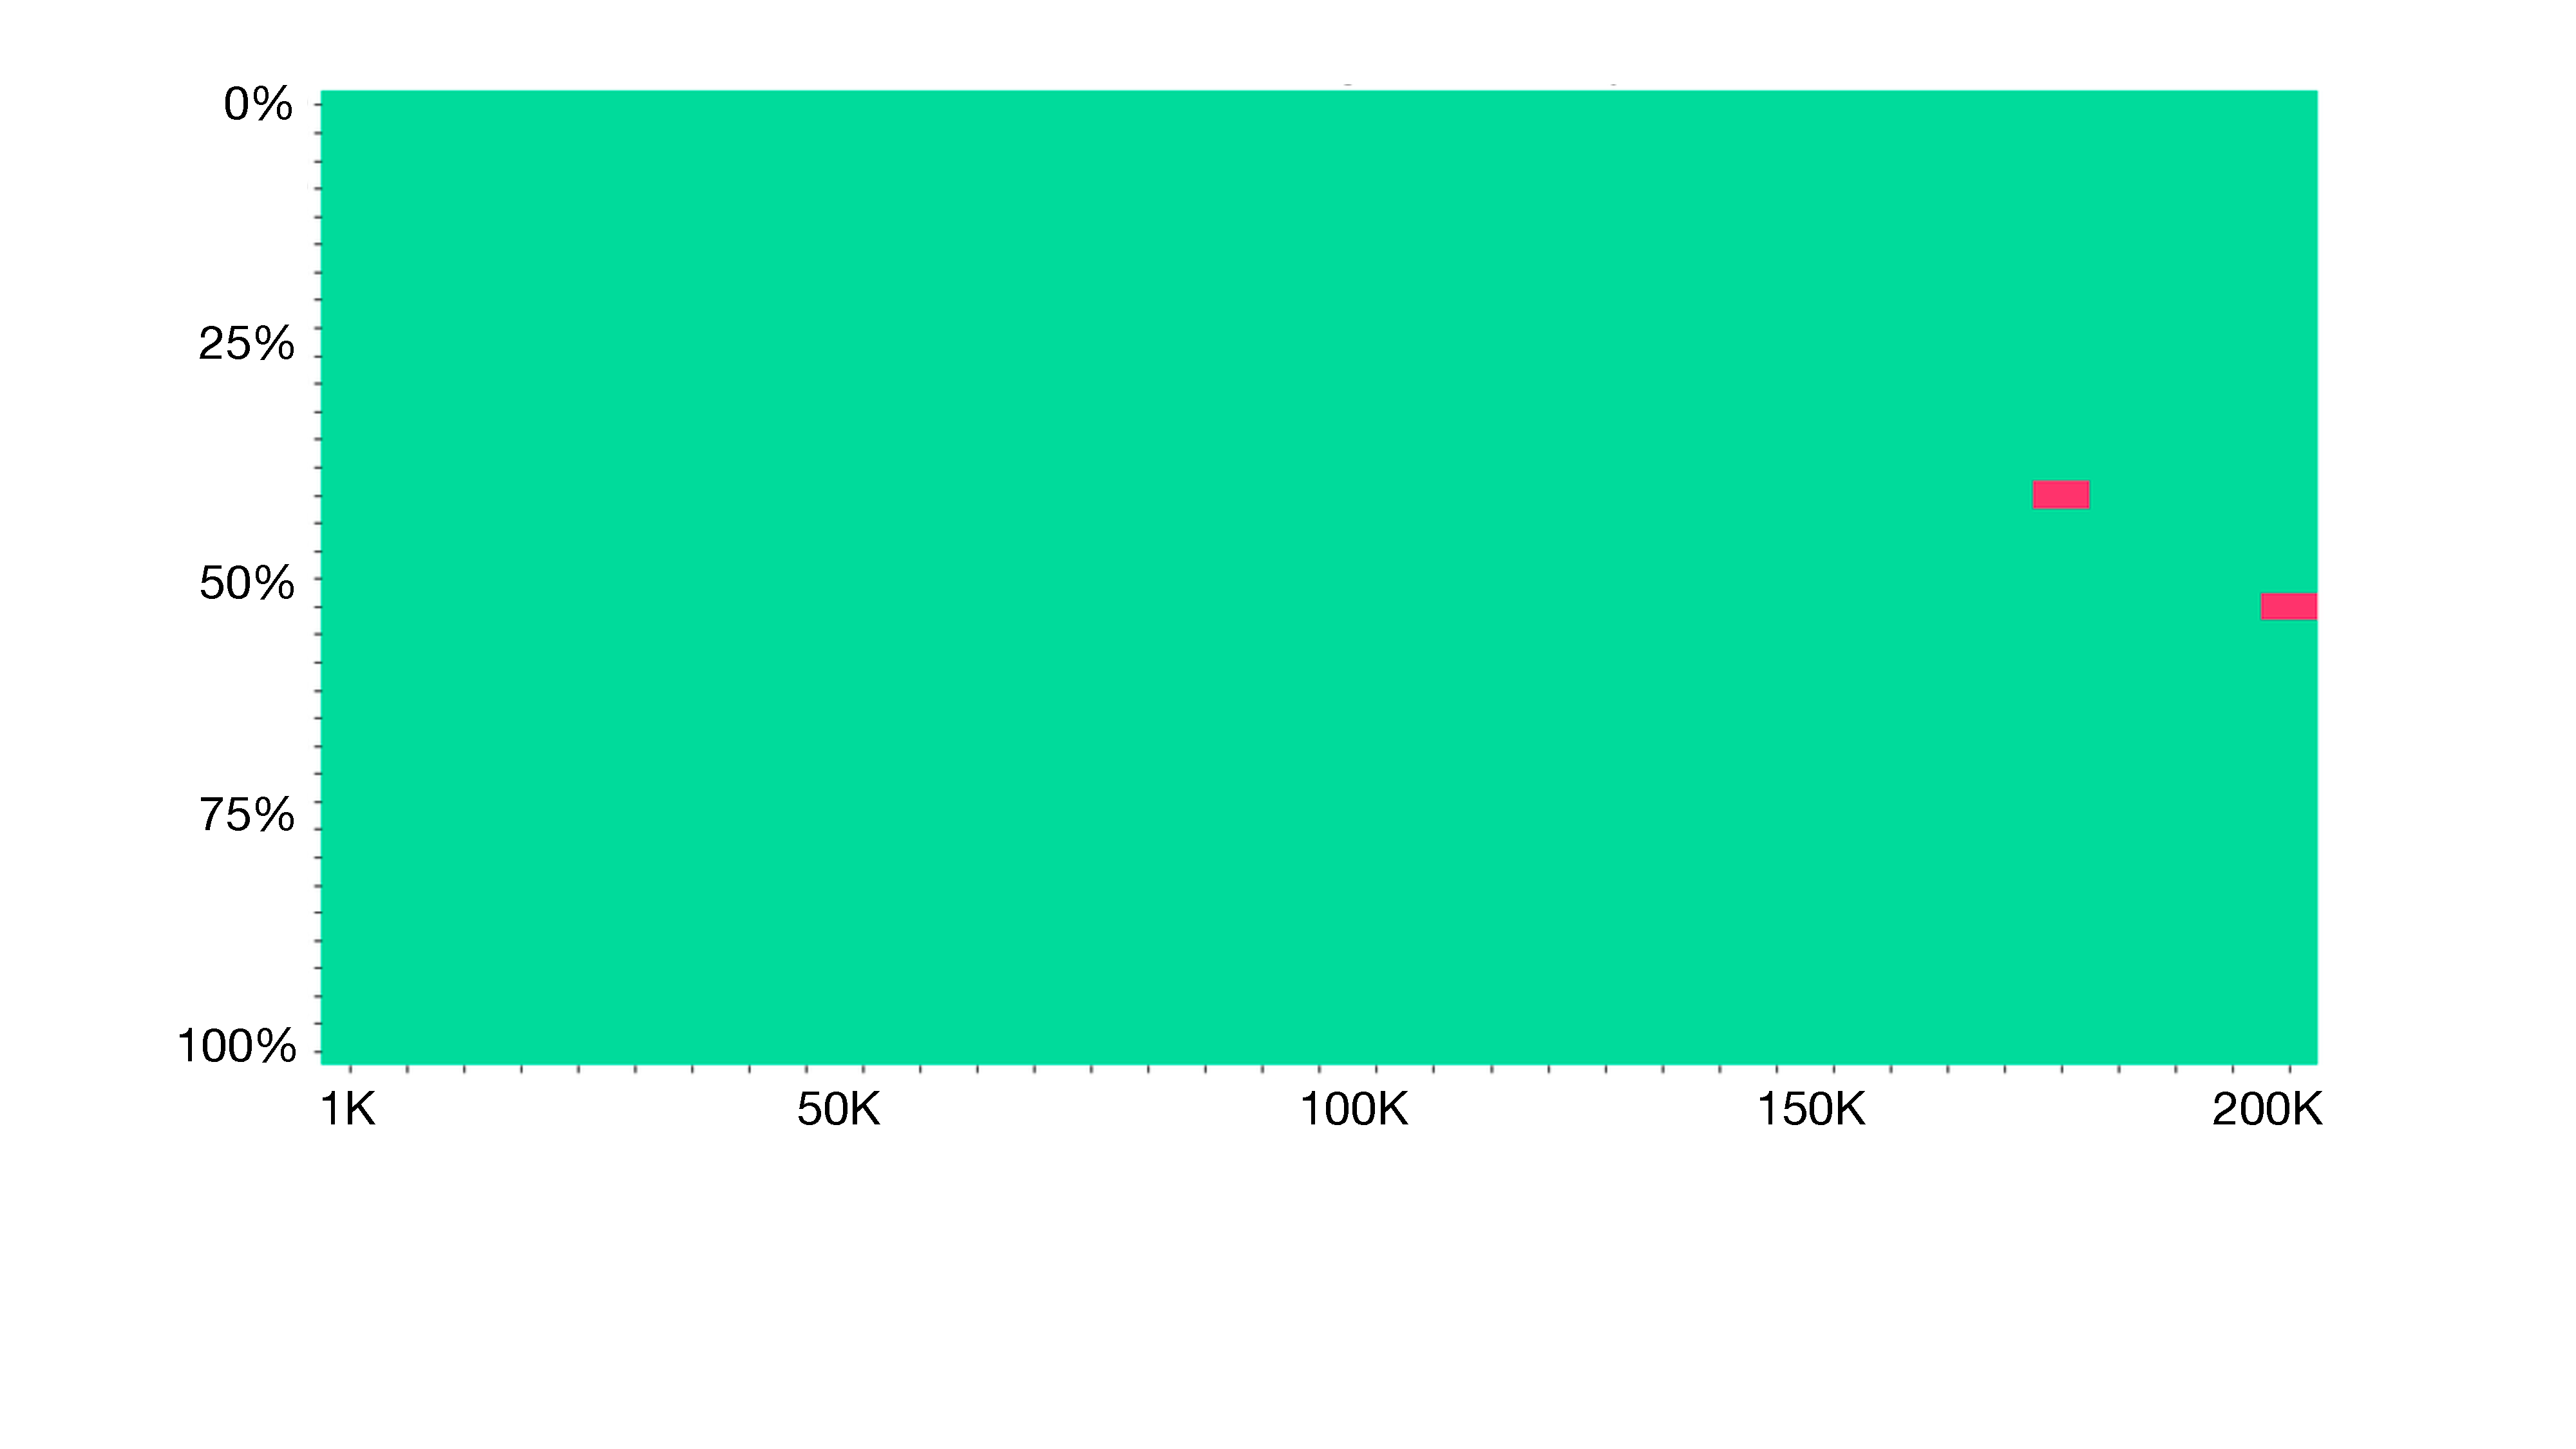
\includegraphics[width=\textwidth]{images/needle.pdf}
	\end{center}
	\caption{Needle-in-a-Haystack performance of Yi-34B-200K. 
        X-axis means length of the document, and Y-axis means the depth of the needle sentence within the document. 
        We continue pretrain the model on 5B tokens long-context data mixture and demonstrates a near-all-green performance.
        } %
	\label{fig:needle}
\end{figure}
\begin{table}[t!]
  \centering
  \begin{tabular}{@{}lccccc@{}}
\toprule
Model   & \bf Average  & \bf Humanity & \bf STEM  & \bf Social Science & \bf Other \\
\midrule
Yi-6B 4K       & 63.24 & 59.10   & 53.15 & 73.83          & 69.26 \\
Yi-6B 200K     & 61.73 & 56.17   & 52.36 & 72.54          & 68.94 \\
Yi-34B 4K      & 76.32 & 73.17   & 68.03 & 85.11          & 80.78 \\
Yi-34B 200K    & 75.56 & 72.20   & 66.83 & 84.76          & 80.40 \\
\bottomrule

  \end{tabular}
   \caption{Performance on MMLU after 200K adaptation. Extending the context length to 200K does not significantly change the short context capability. 
   }
  \label{tab:long_context_mmlu}
\end{table}

The performance of the 200K models is shown in figure.~\ref{fig:needle} and table~\ref{tab:long_context_mmlu}. 
Specifically, Figure~\ref{fig:needle} shows the famous Needle-in-a-Haystack test of Yi-34B-200K, though we tend to view that this level of retrieval is relatively easy for long-context LLMs. 
Table~\ref{tab:long_context_mmlu} shows that our context scaling does not significantly influence the short-context generic capability. 

